\documentclass{article}

\usepackage{tikz}
\usetikzlibrary{automata, positioning, arrows}

\usepackage{geometry}
\geometry {
    top=20mm,
    bmargin=25mm,
}

\begin{document}

\title{ciao}
\author{riciao,  ririciao}
\maketitle

\begin{figure}[ht] % ’ht’ tells LaTeX to place the figure ’here’ or at the top of the page
    \centering % centers the figure

    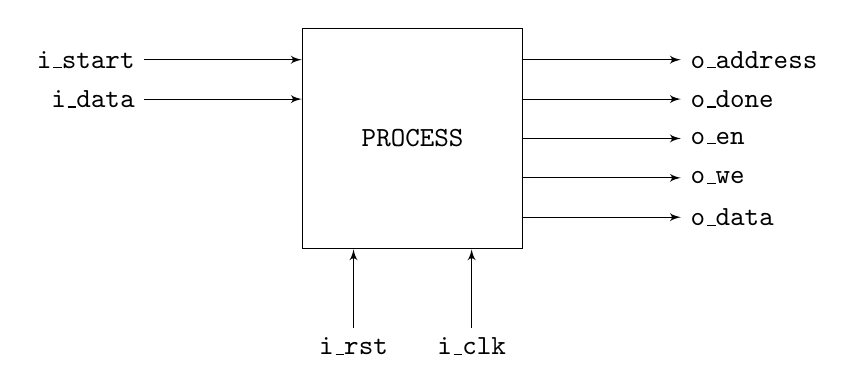
\begin{tikzpicture}[node distance = 5mm and 15mm]
        \node (comp) [draw,minimum size=28mm] {\texttt{PROCESS}};
        % in
        \coordinate[above left= 10mm and 20mm of comp.west]  (i1);
        \foreach \i [count=\xi from 1] in {2} 
            \coordinate[below=of i\xi]  (i\i);
        \foreach \i [count=\xi from 1] in {\texttt{i\_start}, \texttt{i\_data}}
            \draw[-latex']  (i\xi) node[left] {\i} -- (i\xi-| comp.west);
        %under
        \coordinate[below right = 10mm and 7.5mm of comp.south]  (u1);
        \foreach \i [count=\xi from 1] in {2} 
            \coordinate[left=of u\xi]  (u\i);
        \foreach \i [count=\xi from 1] in {\texttt{i\_clk}, \texttt{i\_rst}}
            \draw[-latex']  (u\xi) node[below] {\i} -- (u\xi |- comp.south);
        % out
        \coordinate[above right= 10mm and 20mm of comp.east]  (o1);
        \foreach \i [count=\xi from 1] in {2,...,5} 
            \coordinate[below=of o\xi]  (o\i);
        \foreach \i [count=\xi from 1] in {\texttt{o\_address}, \texttt{o\_done},
                                                    \texttt{o\_en}, \texttt{o\_we}, \texttt{o\_data}}
            \draw[-latex'] (comp.east |- o\xi) -- (o\xi) node[right] {\i};
        %
        \end{tikzpicture}

    \caption{schema del componente realizzato}
    \label{fig:component}
\end{figure}

%\begin{figure}[ht]
%    \centering 
%    \begin{tikzpicture}[->,>=stealth',shorten >=1pt,auto,node distance=3cm,
%        semithick, initial text=$ $, initial where= above]

%        \node[state, initial]           (0) {\texttt{WT\_RST}};
%        \node[state, below of=0]        (1) {\texttt{WT\_STR}};
%        \node[state, below of=1]        (2) {\texttt{RD\_COL}};
%        \node[state, below of=2]        (3) {\texttt{RD\_ROW}};
%        \node[state, below of=3]        (4) {\texttt{CPM\_DT}};
%        \node[state, right=5cm of 3]    (5) {\texttt{RD\_REQ}};
%        \node[state, right=5cm of 4]    (6) {\texttt{WT\_MEM}};
%        \node[state, below of=4]        (7) {\texttt{PREP\_EL}};
%        \node[state, below of=6]        (8) {\texttt{EL\_DATA}};
%        \node[state, left of=7]        (9) {\texttt{DONE}};

%        \draw   (0) edge                        node {\texttt{i\_rst=1}}                                            (1)
%                (1) edge[bend left]             node {\texttt{i\_start=1}}                                          (5)
%                (5) edge                        node {}                                                             (6)
%               (6) edge[bend left=15, right]   node [%yshift=10pt, xshift=-9pt
%                at end, yshift=-15pt, xshift=-35pt] {\texttt{count=0}}                  (2)
%                (6) edge[bend left=20, right]   node [%yshift=6pt, xshift=-5pt
%                at end, yshift=-15pt, xshift=-33pt] {\texttt{count=1}}                   (3)
%                (6) edge                        node [xshift=-20pt] {\texttt{\emph{cond2}}}                         (4)
%                (6) edge                        node {}                                             (8)
%                (2) edge[bend left=15, right]   node {}                                                             (5)
%                (3) edge[bend left=20]          node {\texttt{\emph{cond1}}}                                        (5)
%                (4) edge                        node [at start, yshift=7pt, xshift=25pt] {\texttt{\emph{cond3}}}    (5)
%                (8) edge[bend right]            node[right]  {{\texttt{\emph{cond3}}}} (5)
%                (3) edge[bend right,left]       node {\texttt{\emph{!cond1}}}                                       (9)
%                (4) edge                        node[left] {\texttt{\emph{!cond3}}}                                 (7)
%                (7) edge[bend right=10]         node {}                                                             (5)
%                (8) edge[bend left=25]          node {{\texttt{\emph{!cond3}}}}                                     (9);

%    \end{tikzpicture}
%    \caption{Diagramma degli stati della macchina a stati finiti utilizzata}
%    \label{fig:fsm}
%\end{figure}

\pagebreak

\begin{figure}[ht]
    \centering 
    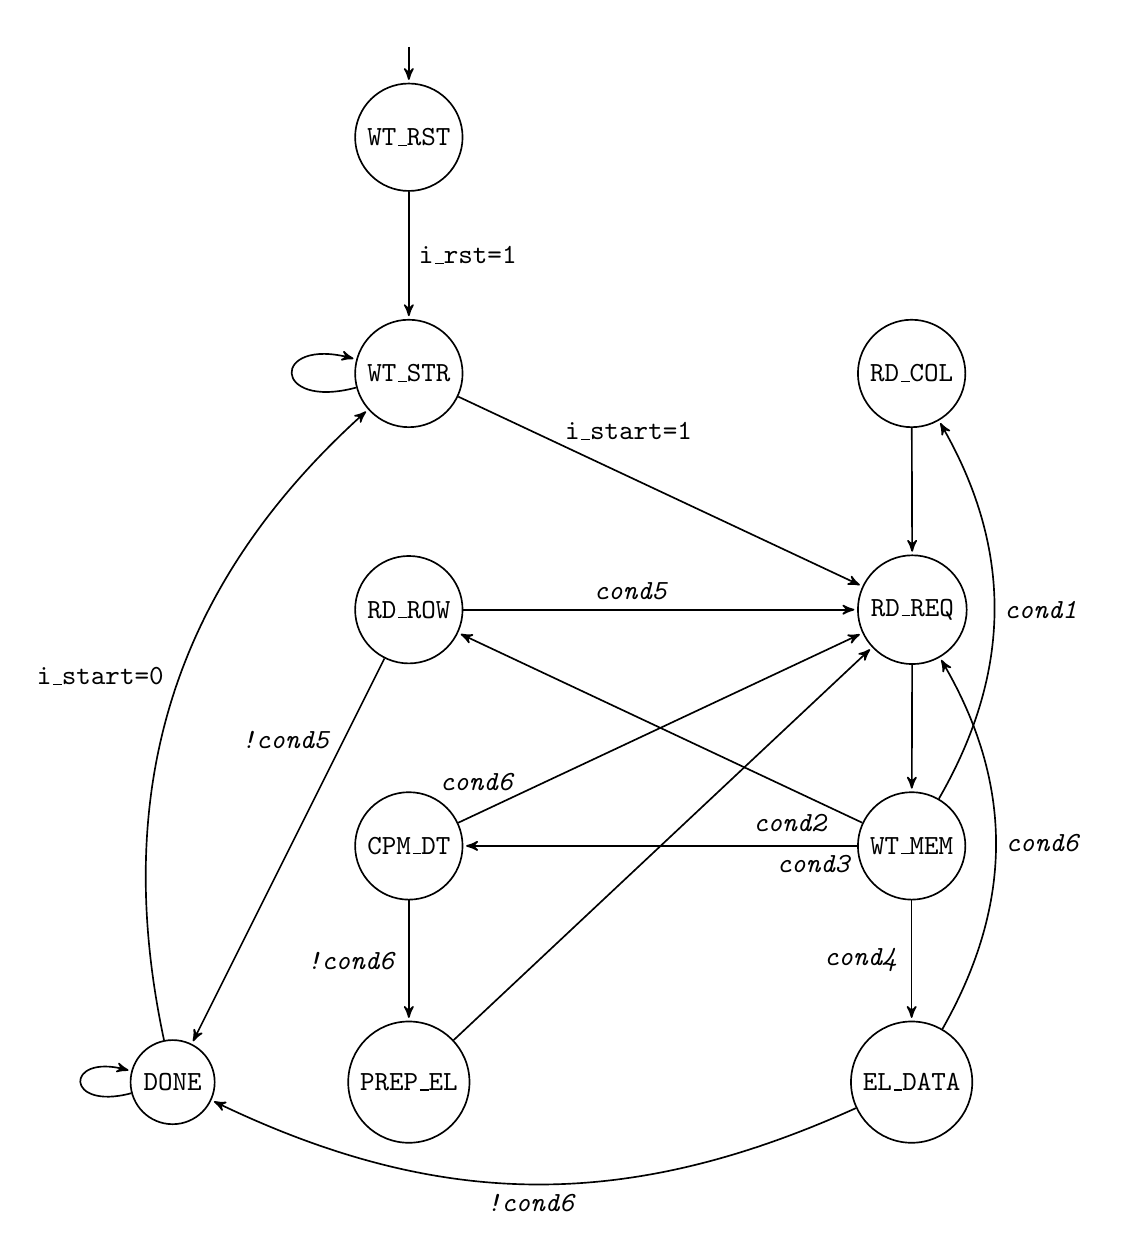
\begin{tikzpicture}[->,>=stealth',shorten >=1pt,auto,node distance=3cm,
        semithick, initial text=$ $, initial where= above]

        \node[state, initial]           (0) {\texttt{WT\_RST}};
        \node[state, below of=0]        (1) {\texttt{WT\_STR}};
        \node[state, right=5cm of 1]    (2) {\texttt{RD\_COL}};
        \node[state, below of=1]        (3) {\texttt{RD\_ROW}};
        \node[state, below of=3]        (4) {\texttt{CPM\_DT}};
        \node[state, right=5cm of 3]    (5) {\texttt{RD\_REQ}};
        \node[state, right=5cm of 4]    (6) {\texttt{WT\_MEM}};
        \node[state, below of=4]        (7) {\texttt{PREP\_EL}};
        \node[state, below of=6]        (8) {\texttt{EL\_DATA}};
        \node[state, left of=7]         (9) {\texttt{DONE}};

        \draw   (0) edge                    node {\texttt{i\_rst=1}}                                            (1)
                
                (1) edge[loop left]                    node {}                                                  (1)
                (1) edge                    node [yshift=15pt, xshift=-38pt]{\texttt{i\_start=1}}               (5)
                
                (2) edge                    node {}                                                             (5)
                
                (3) edge                    node [xshift=-10pt] {\texttt{\emph{cond5}}}                         (5)
                (3) edge[left]   node [yshift=40pt, xshift=20pt]{\texttt{\emph{!cond5}}}                        (9)
                
                (4) edge                    node [at start, yshift=8pt, xshift=25pt] {\texttt{\emph{cond6}}}    (5)
                (4) edge                    node[left] {\texttt{\emph{!cond6}}}                                 (7)
                
                (5) edge                    node {}                                                             (6)
                
                (6) edge[bend right, right] node {\texttt{\emph{cond1}}}                                        (2)
                (6) edge[right]             node [at start, xshift=-43pt] {\texttt{\emph{cond2}}}               (3)
                (6) edge                    node [at start, xshift=-15pt] {\texttt{\emph{cond3}}}               (4)
                (6) edge[left]              node {\texttt{\emph{cond4}}}                                        (8)
                
                (7) edge                    node {}                                                             (5)
                
                (8) edge[bend right]        node[right]  {{\texttt{\emph{cond6}}}}                              (5)
                (8) edge[bend left=25]      node {{\texttt{\emph{!cond6}}}}                                     (9)
                
                (9) edge[bend left]                    node {\texttt{i\_start=0}}                               (1)
                (9) edge[loop left]                    node {}                                                  (9);

    \end{tikzpicture}
    \caption{Diagramma degli stati della macchina a stati finiti utilizzata}
    \label{fig:fsm}
\end{figure}

Le condizioni utilizzate nel processo sono le seguenti:

%\begin{center}
%    \begin{tabular}{ll}
%    \texttt{cond1}: & \texttt{dimImmagine $>$ 0}\\
%    \texttt{cond2}: & \texttt{count $=$ 0} \\
%    \texttt{cond3}: & \texttt{count $=$ 1} \\
%    \texttt{cond4}: & \texttt{dimImmagine $>$ 0} \\
%    \texttt{cond5}: & \texttt{shift\_level $=$ 3 (non ancora calcolato)} \\
%    \texttt{cond6}: & \texttt{count $\leq$ dimImmagine $+$ 2} \\
%    \texttt{cond7}: & \texttt{!cond1 \&\& !cond2 \&\& !cont5} \\    
%    \end{tabular}
%\end{center}

\begin{center}
    \begin{tabular}{||c|c||}
        %\hline
        \hline
        \texttt{\emph{cond1}} & \texttt{count $=$ 0} \\
        \hline
        \texttt{\emph{cond2}} & \texttt{count $=$ 1} \\
        \hline
        \texttt{\emph{cond3}} & \texttt{shift\_level $=$ 3 (non ancora calcolato)} \\
        \hline
        \texttt{\emph{cond4}} & \texttt{\emph{!cond1} \&\& \emph{!cond2} \&\& \emph{!cond3}} \\   
        \hline
        \texttt{\emph{cond5}} & \texttt{n\_col $\cdot$ n\_row $>$ 0} \\
        \hline
        \texttt{\emph{cond6}} & \texttt{count $\leq$ n\_col $\cdot$ n\_row $+$ 2} \\      
        \hline
        %\hline
        \end{tabular}
\end{center}

Si ricorda inoltre, che per ogni stato dell'FSM è presente un arco uscente implicito diretto verso lo stato \texttt{WT\_STR}, 
che simboleggia la possibilità di interrompere in qualsiasi momento l'elaborazione dell'immagine corrente, tramite un segnale \texttt{i\_rst $=$ 1}

\end{document}